\documentclass[hidelinks,a4paper,12pt]{article}
\addtolength{\oddsidemargin}{-1.cm}
\addtolength{\textwidth}{2cm}
\addtolength{\topmargin}{-2cm}
\addtolength{\textheight}{3.5cm}
\newcommand{\HRule}{\rule{\linewidth}{0.5mm}}
\makeindex

\usepackage{longtable}
\usepackage[pdftex]{graphicx}
\usepackage{makeidx}
\usepackage{hyperref}
\hypersetup{
    colorlinks=true,
    linkcolor=black,
    filecolor=magenta,      
    urlcolor=blue,
}


% define the title
\author{Not-Like-This}
\title{ Nimbus Amason Web Services Network Visualiser User Manual}
\begin{document}
\setlength{\parskip}{6pt}

% generates the title
\begin{titlepage}

\begin{center}
% Upper part of the page       

\includegraphics[width=1\textwidth]{./images/up-logo.jpg}\\[0.4cm]    
\textsc{\LARGE Department of Computer Science}\\[1.5cm]
\textsc{\Large COS 301 - Software Engineering}\\[0.5cm]
% Title
\HRule \\[0.4cm]

\includegraphics[width=0.05\textwidth]{./images/logo.png}
{ \huge \bfseries Nimbus}

\includegraphics[width=0.05\textwidth]{./images/logo.png}\\[0.4cm]   
{ \huge \bfseries User Manual}\\[0.4cm]
\HRule \\[0.4cm]
% Author and supervisor
\textsc{\Large Men-At-Work}\\[0.5cm]
\begin{minipage}{0.4\textwidth}
\begin{flushleft} \large
\emph{Authors:}
\end{flushleft}
\end{minipage}
\begin{minipage}{0.4\textwidth}
\begin{flushright} \large
\emph{Student number:}
\end{flushright}
\end{minipage}

\begin{minipage}{0.4\textwidth}
\begin{flushleft} \large
Jedd {Schneier}
\end{flushleft}
\end{minipage}
\begin{minipage}{0.4\textwidth}
\begin{flushright} \large
\emph{}
u13133064
\end{flushright}
\end{minipage}

\begin{minipage}{0.4\textwidth}
\begin{flushleft} \large
Daniel {King}
\end{flushleft}
\end{minipage}
\begin{minipage}{0.4\textwidth}
\begin{flushright} \large
\emph{}
u13307607
\end{flushright}
\end{minipage}

\begin{minipage}{0.4\textwidth}
\begin{flushleft} \large
Muller {Potgieter}
\end{flushleft}
\end{minipage}
\begin{minipage}{0.4\textwidth}
\begin{flushright} \large
\emph{}
u12003672
\end{flushright}
\end{minipage}
\vfill
% Bottom of the page
{\large \today}
\end{center}
\end{titlepage}
\footnotesize
%\input{declaration_of_originality.tex}
\normalsize


\pagenumbering{roman}
\tableofcontents
\newpage
\pagenumbering{arabic}

\newpage
\section{System Overview} 

Nimbus, the Amazon Web Services (AWS) network visualiser, will by usable by registered users of AWS. The system will scan the AWS network and build a visual hierarchy, so that the user may have a better understanding of the network's structure, how different services relate to each other and gain information in an intuitive manner. After opening the web page, the user must log in using their AWS access- and secret key. Only once the user's identity has been verified by our server, will it allow them to make use of Nimbus. Once the user has succesfully logged in, they may begin the network scan. The browser itself does not scan the AWS, rather it communicates with our server. The user may choose to simply scan their network in its entirety, or only to scan certain parts of it. Our server scans and maps out the network, then sends the relevant information to the browser. The browser processes this and displays the hierarchy.


\section{System Configuration}
\begin {itemize}
	\item The user will use a browser to make use of the webpage and the server.
	\item The user requires internet access in order to make use of the server and its scanning capabilities. 
	\item The web page does offer the ability to store and load .json files, which are representative of the current scan.
\end{itemize}


\newpage

\section{Installation}
\begin {enumerate}
	\item The user must go on GitHub ( \url {https://github.com/u13133064/NotLikeThis/tree/master/Main/NotLikeThisRESTServer}) and download the project files onto their PC.
	\begin{center}
  		 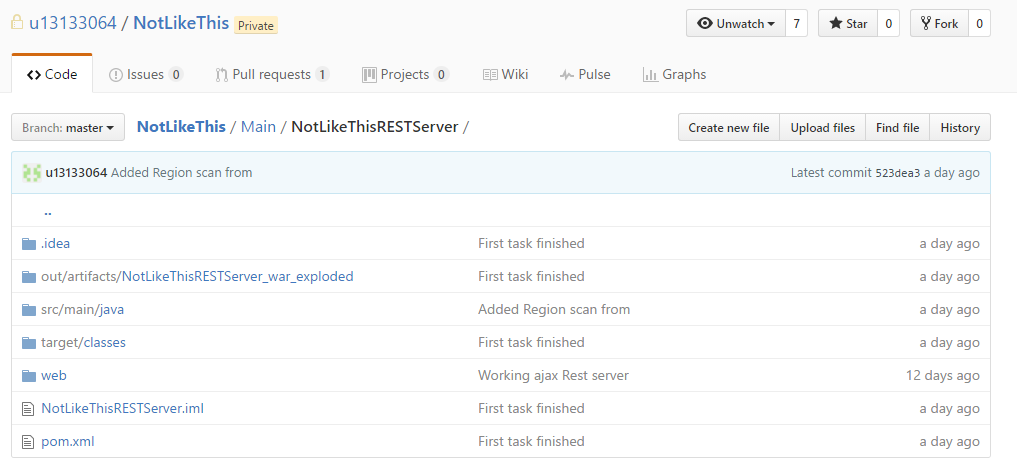
\includegraphics[width=0.9\textwidth] {./images/Github.png}\\[0.4cm]
	\end{center}
	
	\item The user must have Java EE installed.
	\item The user must have IntelliJ Developer Edition installed.
	\item The user must follow the steps specified in the next two blogs to get a working server.
	\item ( \url {http://jason.zwolak.org/technoblog/2013/06/restful-service-with-tomee-and-intellij-idea/})
	\item ( \url {https://chiaboy.wordpress.com/2014/07/20/simple-jersey-example-with-intellij-idea-and-tomcat/})
		\begin{center}
			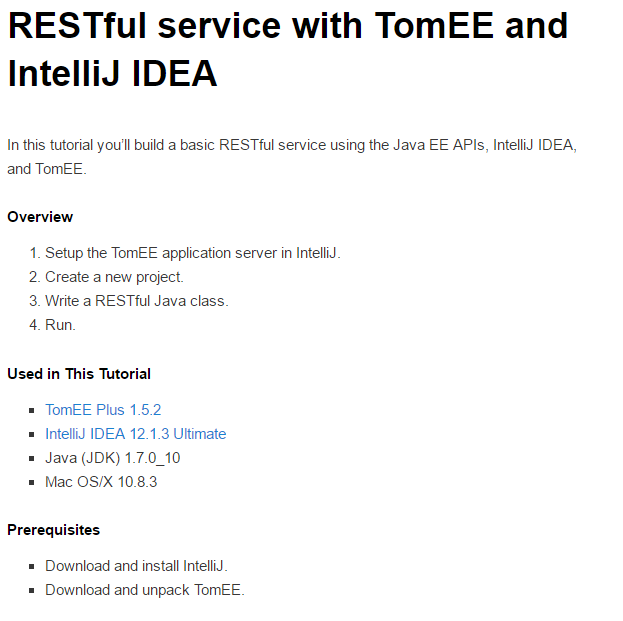
\includegraphics[width=0.3\textwidth] {./images/InstallOne.png}\\[0.4cm]
	
					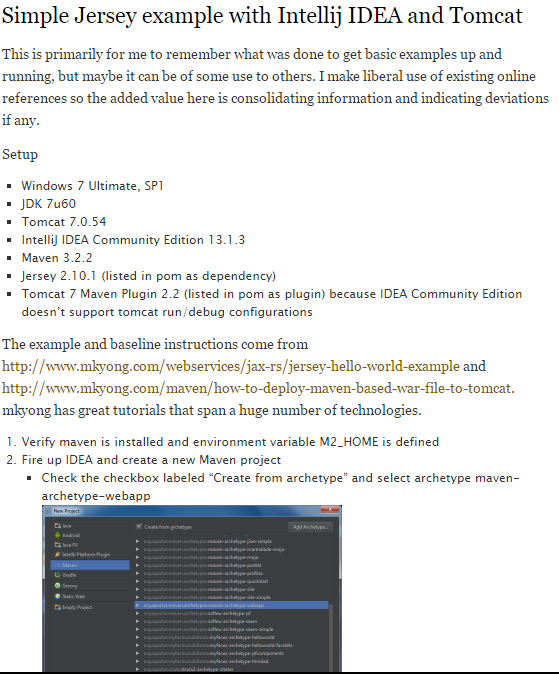
\includegraphics[width=0.3\textwidth] {./images/InstallTwo.png}\\[0.4cm]
				\end{center}

	
	
	
\end{enumerate}

\newpage

\section{Getting started}
	\begin {itemize}
		\item In order to make use of Nimbus, the user must already be a registered AWS user.
		\item The user's password and secret password are provided by AWS.
		\item Once the user has logged in, they can make full use of Nimbus.
		\item Once they are done, they may choose to log out of Nimbus, ending their session.
	\end{itemize}

\newpage

\section{Using the system}
The functionality of the visualiser is spread between the following use cases:

	\subsection{Login}
		\begin {itemize}
			\item The user is presented with two options for logging in. The first is to enter their details into the input boxes at the top of the web page, Access Key and Secret Key.
			\item Once the details are filled in, pressing "Login" will log the user into the server.
		\end{itemize}
		
  		\begin{center}
    			
\includegraphics[width=0.7\textwidth]{./images/LoginOne.png}
  		\end{center}

		\begin {itemize}
		\item The second option is to immediately press the  "Scan Network" button.
		\item If this occurs, the user is presented with an alert box, where they may enter their Access Key and Secret Key.
		\end{itemize}
		
		\begin{center}
			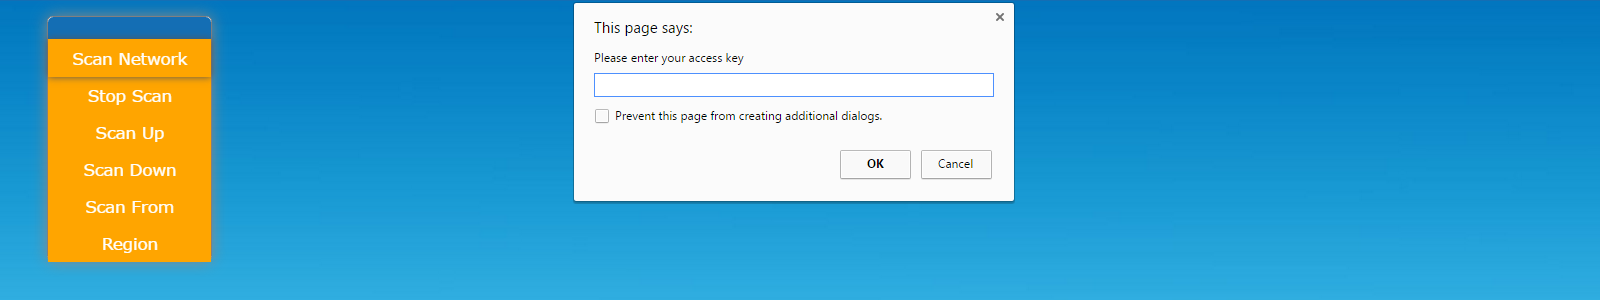
\includegraphics[width=0.9\textwidth]{./images/LoginTwo.png}
		\end{center}
		

	\subsection{Logout}
		\begin {itemize}
			\item Once the user has finished their session, they can log out using the "Logout" button.
		\end{itemize}
	\newpage
	
	\subsection{Scan Network}
		\begin {itemize}
			\item After the user has successfully logged in, they may scan the network, by pressing "Scan Network".
			\item The network will then build a hierarchial tree node by node, so that the user may follow its construction with ease.
			\item The network presented here is for demonstration purposes and is not reflective of an actual network.
		\end{itemize}
		\begin{center}
			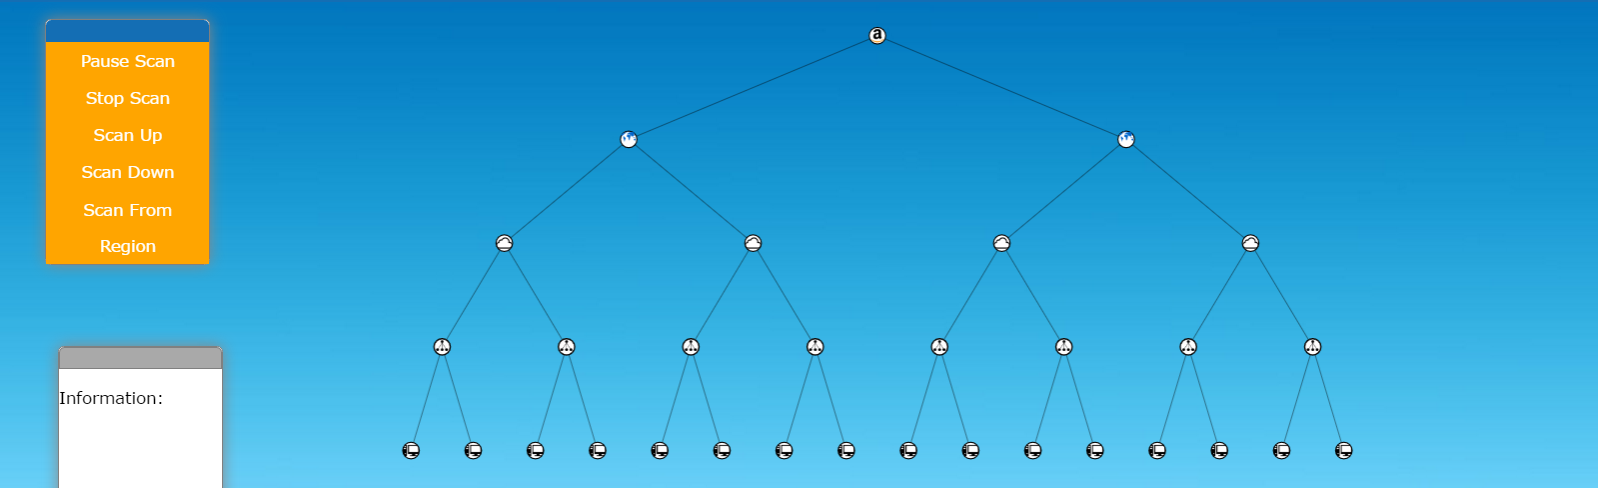
\includegraphics[width=0.9\textwidth]{./images/PostScanLaunch.png}
			\end{center}	
		
	
		
	\subsection{Pause/Resume}
	\begin {itemize}
	\item While the scan is active, it can be paused.It will halt the scan's execution, but it can be resumed.
	\item While the scan is is inactive, it can be resumed. This will resume scan's execution, from where it left off
	\end{itemize}
	
	\begin{center}
		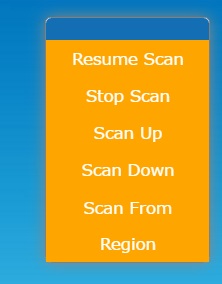
\includegraphics[width=0.45\textwidth]{./images/AfterPause.png}
		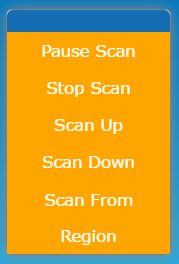
\includegraphics[width=0.4\textwidth]{./images/WhileActive.png}
	\end{center}	
	
	\newpage
	
		\subsection{Stop}
		\begin {itemize}
		\item If the scan is stopped, a new scan may be begun. Progress from the previous scan is lost.
	\end{itemize}
	
	\begin{center}
		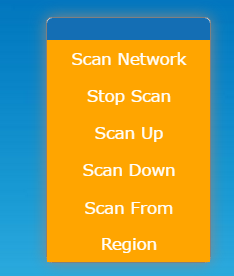
\includegraphics[width=0.45\textwidth]{./images/AfterStop.png}
	\end{center}	

	
	\subsection{Scan up/down}
			\begin {itemize}
			\item Selecting "Scan Up" or "Scan Down" will determine the direction the scan is goes.
	\end{itemize}
		
		\newpage
		
			\subsection{Regions}
			\begin {itemize}
			\item Hovering the mouse over "Region" will reveal a drop-down list with all the AWS regions. 
			\item Selecting a region will cause the scan to only scan nodes that fall under the selected region.
		\end{itemize}
		
		\begin{center}
			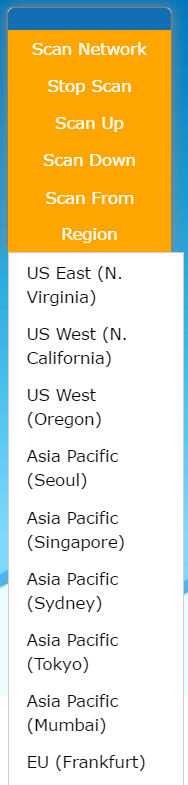
\includegraphics[width=0.3\textwidth]{./images/RegionSelect.png}

		\end{center}	
		
		\newpage
		
		
		\subsection{Zooming}
			\begin {itemize}
			\item Hovering the mouse over the hierarchy and rolling the mouse forwards or backwards will zoom in and zoom out respectively.
		\end{itemize}
		
		\begin{center}
			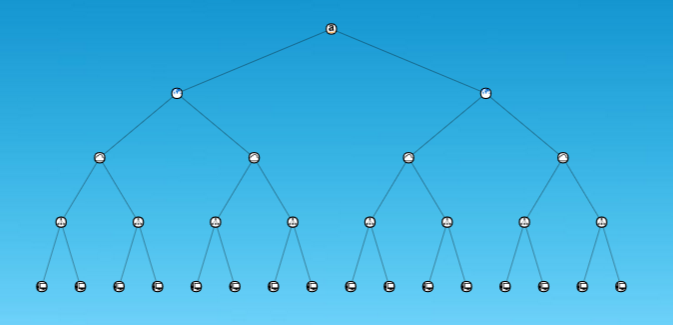
\includegraphics[width=0.45\textwidth]{./images/ZoomOut.png}
			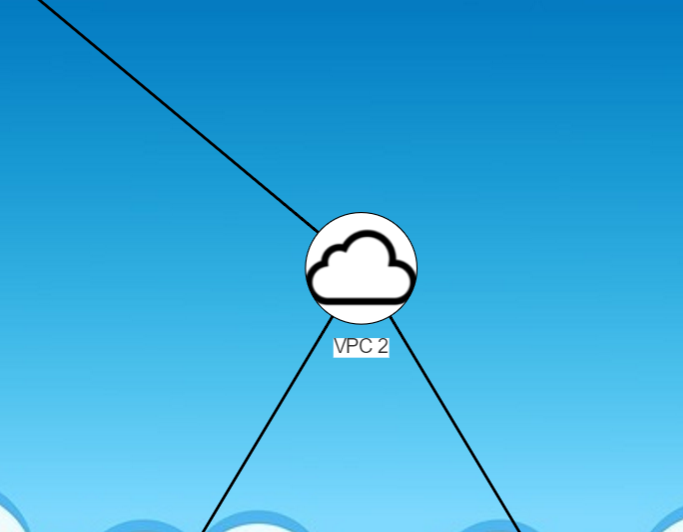
\includegraphics[width=0.3\textwidth]{./images/ZoomIn.png}
		\end{center}	
		
				\subsection{Dragging}
				\begin {itemize}
				\item Clicking and holding the mouse over the hierarchy allows the user to move the tree around the screen.
				\item While this occurs, edges are not displayed. This is for effeciency's sake.
			\end{itemize}
			
			\begin{center}
				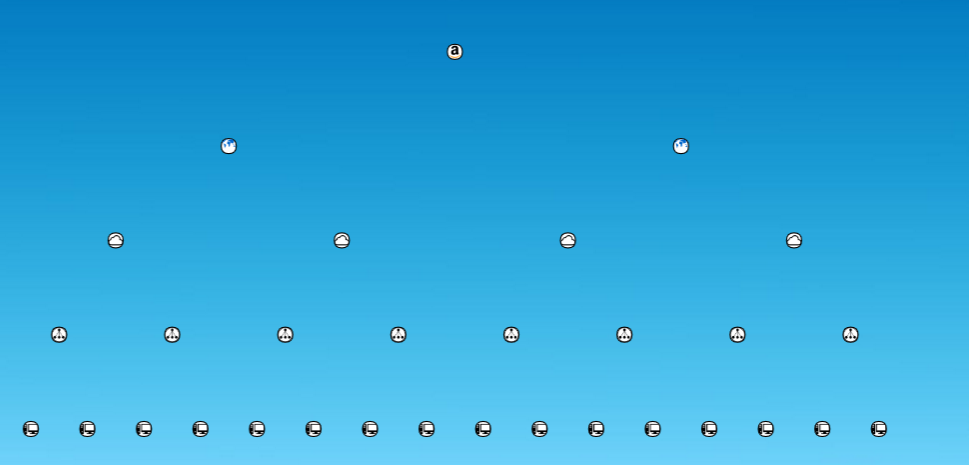
\includegraphics[width=0.45\textwidth]{./images/Dragging.png}

			\end{center}
		
			\subsection{Hovering over a node}
						\begin {itemize}
						\item Hovering the mouse over a node will highlingt it and its edges
					\end{itemize}
					
					\begin{center}
						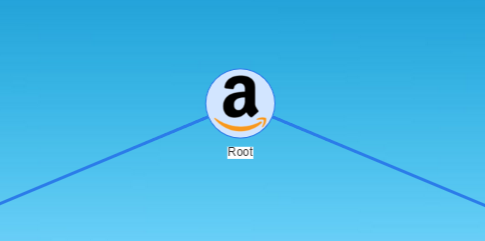
\includegraphics[width=0.45\textwidth]{./images/NodeHover.png}
						
					\end{center}
		\newpage
		
		\subsection{Clicking on a node}
					\begin {itemize}
					\item Clicking on a node will turn its and its border's black.
					\item When a node is clicked, the server is queried and its information is loaded into the grey box.
				\end{itemize}
				
				\begin{center}
					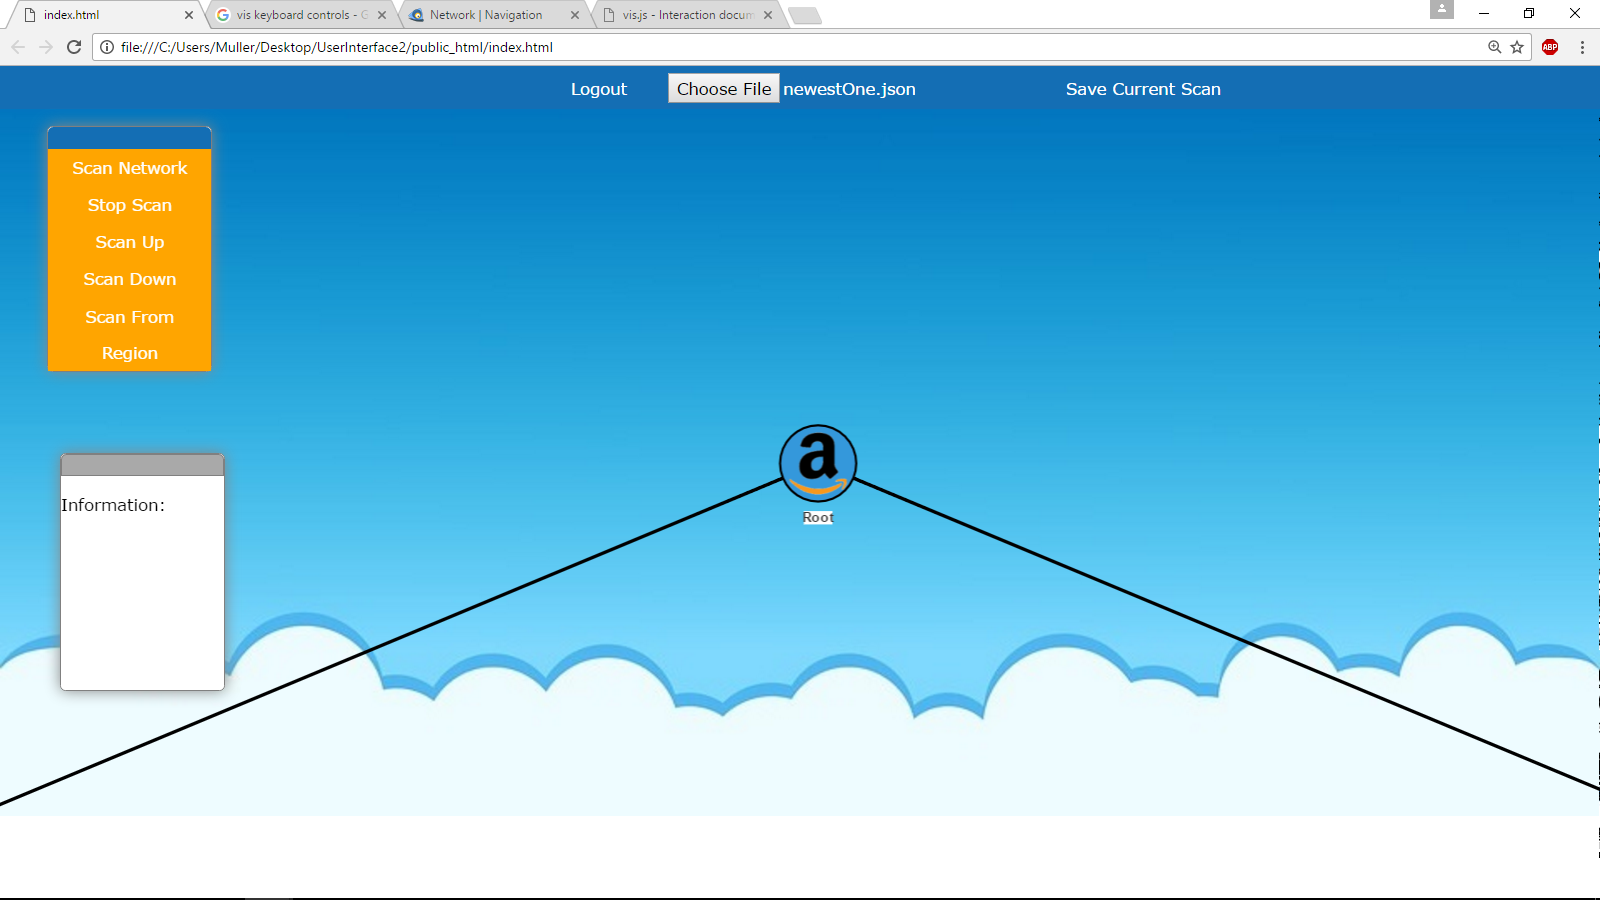
\includegraphics[width=0.45\textwidth]{./images/SelectNode.png}
					
				\end{center}
		
		\subsection{Dragging boxes}
				\begin {itemize}
				\item The box containing the network controls and the box where node information is displayed, can be moved.
				\item The small bar at the top of both boxes can be dragged, allowing for ease of use
			\end{itemize}
			
			\begin{center}
				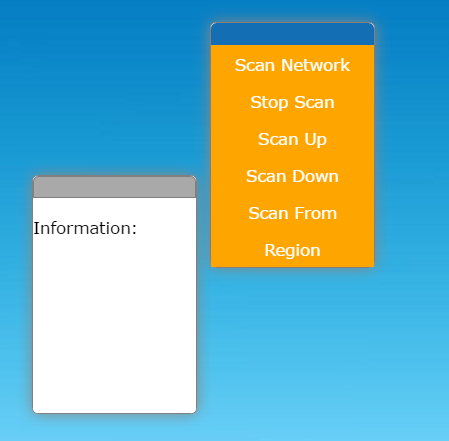
\includegraphics[width=0.45\textwidth]{./images/DragBoxes.png}
				
			\end{center}
			\newpage	
			
			\subsection{Loading from a file}
					\begin {itemize}
					\item The web page provides an offline option, where the user may choose to load a file from a previous session. 
					\item This will not allow the user to gain information from the node, as a node's information is stored online.
				\end{itemize}
				
				\begin{center}
					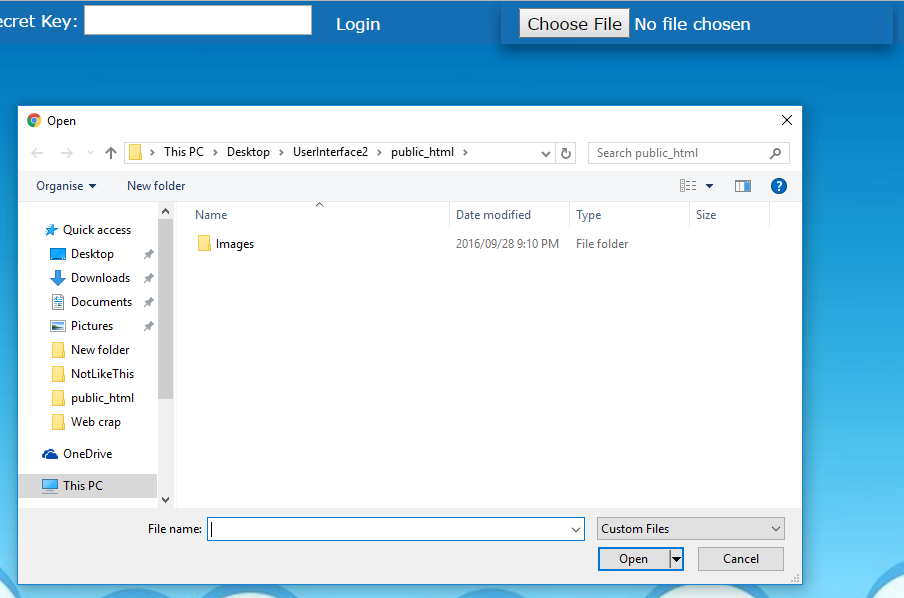
\includegraphics[width=0.8\textwidth]{./images/OpenFile.png}
				\end{center}
			
				
				\subsection{Saving a file}
				\begin {itemize}
				\item Clicking "Save Current Scan" will store the current scan into a .json file, that can be loaded by the web page 
			\end{itemize}
			
	\begin{center}
		
\includegraphics[width=0.8\textwidth]{./images/FileInteractions.png}
	\end{center}
				
					\newpage
							
								
	
	
\section{Troubleshooting}
	In the event that an error occurs, the user will be presented with a comprehensive error message. If the error is with the browser or the web page, it is displayed as an alert box. If the error is on the server side, an error will be thrown. If the server experiences an error while the browser is active, an error message will display, to explain what occurred.
		
\end{document}
